\documentclass[main.tex]{subfiles}
%% Current Author: PS
\setcounter{chapter}{3}
\begin{document}
\chapter{Energy Concepts}
\raggedbottom
\begin{content}
    \item work
    \item power
    \item potential and kinetic energy
    \item energy conversion and conservation
    \item specific latent heat
\item specific heat capacity
\end{content}

\section*{Candidates should be able to}

\spec{understand and use the concept of work in terms of the product of a force and a displacement in the direction of that force, including situations where the force is not along the line of motion}

Work, in a scientific sense, is done whenever a force, $F$ acts on an object which moves through a displacement $s$. When the force and the displacement are acting along the same line then work is simply calculated using $W=Fs$. However, when the force does not act in the same direction as the displacement, the work done is calculated by multiplying the component of the force in the direction of the displacement by the displacement as shown in figure \ref{work}.

\begin{figure}[h]
  \begin{center}
    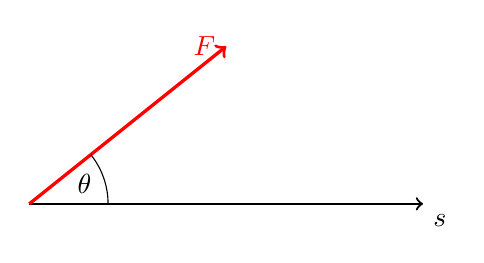
\begin{tikzpicture}
      \draw[thick, ->] (0,2) -- (5,2) node[anchor=north west] {$s$};
      \draw[very thick, ->, red] (0,2) -- (2.5,4) node[anchor=east] {$F$};
      \draw (1,2) arc [start angle=0, end angle=38.66, radius=1cm];
      \draw (.7,2.5) node[anchor=north] {$\theta$};
    \end{tikzpicture}
  \end{center}
  \caption{Non-aligned force doing work}
  \label{work}
\end{figure}

In this case the work done is given by
 \begin{equation}\label{eq:work}
 W = Fs\cos{\theta}
 \end{equation}.

Note that this means that the following cases work is \emph{not} done:
\begin{itemize}
  \item any stationary object (no displacement);
  \item an object in circular motion (the force is acting at right angles to the displacement).
\end{itemize}

Whenever work is done energy is transferred to or from the object. The type of energy this is transferred to or from varies depending on the circumstances.

\spec{calculate the work done in situations where the force is a function of displacement using the area under a force-displacement graph}

Equation \ref{eq:work} applies whenever a constant force acts over a displacement; however, if the force varies then a different approach is needed. Force a constant force acting in the same direction as the displacement, it can be seen that the area under a force-displacement graph is equal to $Fs$, i.e. the work done. This is generally true and work can be written in an integral form as:
\begin{equation}\label{eq:work-integral}
  W = \int F \ud s
\end{equation}

\begin{figure}[h]
  \begin{center}
    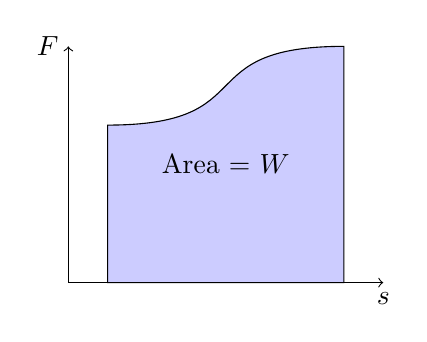
\begin{tikzpicture}
      \draw[<->] (0,3) node[anchor=east] {$F$} -- (0,0) -- (4,0) node[anchor=north] {$s$};
      \filldraw[fill=blue!20!white] (.5,0) -- (.5,2) .. controls (2.5,2) and (1.5,3) .. (3.5,3) -- (3.5,0) -- cycle;
      \draw (2,1.5) node {Area = $W$};
    \end{tikzpicture}
  \end{center}
  \caption{Work as area under a graph}
  \label{fig:work-graph}
\end{figure}

\spec{understand that a heat engine is a device that is supplied with thermal energy and converts some of this energy into useful work}

A heat engine is a device which uses heat to do work. This is shown schematically in figure \ref{fig:heat}. The energy for the work done comes from the difference between $Q_1$ and $Q_2$.
Examples of heat engines include internal combustion engines, jet engines and steam turbines.

\begin{figure}[h]
  \begin{center}
    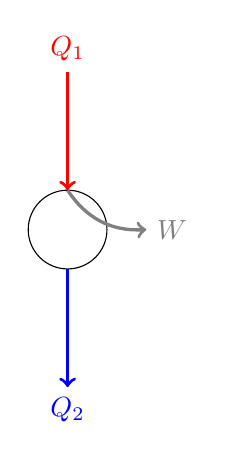
\begin{tikzpicture}
      \draw[very thick, red, ->] (0,2) node[anchor=south] {$Q_1$} -- (0,.5);
      \draw (0,0) circle (.5cm);
      \draw[bend right, very thick, gray, ->] (0,.5) to (1,0) node[anchor=west] {$W$};
      \draw[very thick, blue, ->] (0,-.5) -- (0,-2) node[anchor=north] {$Q_2$};
    \end{tikzpicture}
  \end{center}
  \caption{A heat engine}
  \label{fig:heat}
\end{figure}

\spec{calculate power from the rate at which work is done or energy is transferred}

Power is defines as the rate at which energy is transferred and is measured in watts (\si{\watt}).
\begin{equation}\label{eqn:power}
  P = \frac{W}{t}
\end{equation}

\spec{recall and use $P = Fv$}

For a constant force, this equation can be shown from equation \ref{eqn:power} and \ref{eq:work}:
\[ P = \frac{W}{T} = F\ \frac{s}{t} = Fv \]

\spec{recall and use $\Delta E = mg\Delta h$ for the gravitational potential energy transferred near the Earth's surface}

This is familiar from GCSE.

\spec{recall and use $g\Delta h$ as change in gravitational potential}

Gravitational potential is defined as the energy per init mass. Hence, the change in gravitational potential is given by \[\frac{mg\Delta h}{m} = g\Delta h\]

\spec{recall and use $E = \frac{1}{2}Fx$ for the elastic strain energy in a deformed material sample obeying Hooke's law}
\spec{use the area under a force-extension graph to determine elastic strain energy}

This relies on equating the work done straining an object with the elastic strain energy stored in the object. Once is is done, the statement follows from equation \ref{eq:work-integral} and figure \ref{fig:work-graph}.

The area of such a graph when the material obeys Hooke's Law is $\frac{1}{2}Fx$.

\begin{figure}[h]
  \begin{center}
    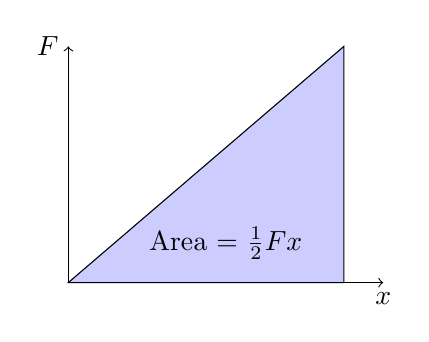
\begin{tikzpicture}
      \draw[<->] (0,3) node[anchor=east] {$F$} -- (0,0) -- (4,0) node[anchor=north] {$x$};
      \filldraw[fill=blue!20!white] (0,0) -- (3.5,3) --(3.5,0) -- cycle;
      \draw (2,.5) node {Area = $\frac{1}{2}Fx$};
    \end{tikzpicture}
  \end{center}
  \caption{Work as area under a graph}
  \label{fig:hooke's law}
\end{figure}

\spec{derive, recall and use $E=\frac{1}{2}kx^2$}

This can be arrived at from Hooke's Law ($F=kx$) and the definition of work in equation \ref{eq:work-integral}, noticing that the extension of the spring is equal to the displacement of the object.
\[ W = \int F \ud s = \int_0^x kx \ud x = \frac{1}{2}kx^2 \]

This integration could equally be done by substituting $F=kx$ into the expression for elastic strain energy derived above from the graph.

\spec{derive, recall and use $E=\frac{1}{2}mv^2$ for the kinetic energy of a body}

Consider the work done accelerating an object from rest to a velocity $v$. Using the equations for uniform accleration with $u=0$ we can see that

\[ W = Fs = mas = m\ \frac{v}{t}\ \frac{v}{2}\ t = \frac{1}{2}mv^2 \]

Since this work has gone into the kinetic energy of the object this formula gives us this kinetic energy.

\spec{apply the principle of conservation of energy to solve problems}

The principle of conservation of energy states that energy cannot be created or destroyed, only transferred between different forms.

\spec{recall and use \[\%\  \text{efficiency} = \frac{\text{useful energy (or power) out}}{\text{total energy (or power) in}} \times 100\]}

This is familiar from GCSE.

\spec{recognise and use $\Delta E = mc \Delta\theta$, where c is the specific heat capacity}

The specific heat capacity is defined as the energy required to heat \SI{1}{\kilo\gram} of a substance by \SI{1}{\celsius}.

\begin{example}
  A kettle with a power rating of \SI{2}{\kilo\watt} heats \SI{500}{\gram} of water from \SI{15}{\celsius} to boiling. If the kettle is 80\% efficient, calculate the time take for the water to boil.

  The specific heat capacity of water is \SI{4200}{\joule\per\kilogram\per\celsius}

  \answer

  Total heat energy required by the water:
  \[ \Delta E = \SI{0.5}{\kilogram} \times \SI{4200}{\joule\per\kilogram\per\celsius} \times \SI{85}{\celsius} = \SI{178.5}{\kilo\joule} \]

  Useful power provided by the kettle:

  \[ P = 0.8 \times \SI{2}{\kilo\watt} = \SI{1.6}{\kilo\watt} \]

  Therefore the time taken is:
  \[ t = \frac{\Delta E}{P} = \frac{\SI{178.5}{\kilo\joule}}{\SI{1.6}{\kilo\watt}} = \SI{112}{\second} \]

\end{example}

\spec{recognise and use $\Delta E = mL$, where L is the specific latent heat of fusion or of vaporisation}

When a substance changes state it releases or absorbs energy. This energy is known as the latent head. The specific latent heat is the energy absorbed or released when \SI{1}{\kilogram} of the substance changes state.


\end{document}
